\documentclass[1p]{elsarticle_modified}
%\bibliographystyle{elsarticle-num}

%\usepackage[colorlinks]{hyperref}
%\usepackage{abbrmath_seonhwa} %\Abb, \Ascr, \Acal ,\Abf, \Afrak
\usepackage{amsfonts}
\usepackage{amssymb}
\usepackage{amsmath}
\usepackage{amsthm}
\usepackage{scalefnt}
\usepackage{amsbsy}
\usepackage{kotex}
\usepackage{caption}
\usepackage{subfig}
\usepackage{color}
\usepackage{graphicx}
\usepackage{xcolor} %% white, black, red, green, blue, cyan, magenta, yellow
\usepackage{float}
\usepackage{setspace}
\usepackage{hyperref}

\usepackage{tikz}
\usetikzlibrary{arrows}

\usepackage{multirow}
\usepackage{array} % fixed length table
\usepackage{hhline}

%%%%%%%%%%%%%%%%%%%%%
\makeatletter
\renewcommand*\env@matrix[1][\arraystretch]{%
	\edef\arraystretch{#1}%
	\hskip -\arraycolsep
	\let\@ifnextchar\new@ifnextchar
	\array{*\c@MaxMatrixCols c}}
\makeatother %https://tex.stackexchange.com/questions/14071/how-can-i-increase-the-line-spacing-in-a-matrix
%%%%%%%%%%%%%%%

\usepackage[normalem]{ulem}

\newcommand{\msout}[1]{\ifmmode\text{\sout{\ensuremath{#1}}}\else\sout{#1}\fi}
%SOURCE: \msout is \stkout macro in https://tex.stackexchange.com/questions/20609/strikeout-in-math-mode

\newcommand{\cancel}[1]{
	\ifmmode
	{\color{red}\msout{#1}}
	\else
	{\color{red}\sout{#1}}
	\fi
}

\newcommand{\add}[1]{
	{\color{blue}\uwave{#1}}
}

\newcommand{\replace}[2]{
	\ifmmode
	{\color{red}\msout{#1}}{\color{blue}\uwave{#2}}
	\else
	{\color{red}\sout{#1}}{\color{blue}\uwave{#2}}
	\fi
}

\newcommand{\Sol}{\mathcal{S}} %segment
\newcommand{\D}{D} %diagram
\newcommand{\A}{\mathcal{A}} %arc


%%%%%%%%%%%%%%%%%%%%%%%%%%%%%5 test

\def\sl{\operatorname{\textup{SL}}(2,\Cbb)}
\def\psl{\operatorname{\textup{PSL}}(2,\Cbb)}
\def\quan{\mkern 1mu \triangleright \mkern 1mu}

\theoremstyle{definition}
\newtheorem{thm}{Theorem}[section]
\newtheorem{prop}[thm]{Proposition}
\newtheorem{lem}[thm]{Lemma}
\newtheorem{ques}[thm]{Question}
\newtheorem{cor}[thm]{Corollary}
\newtheorem{defn}[thm]{Definition}
\newtheorem{exam}[thm]{Example}
\newtheorem{rmk}[thm]{Remark}
\newtheorem{alg}[thm]{Algorithm}

\newcommand{\I}{\sqrt{-1}}
\begin{document}

%\begin{frontmatter}
%
%\title{Boundary parabolic representations of knots up to 8 crossings}
%
%%% Group authors per affiliation:
%\author{Yunhi Cho} 
%\address{Department of Mathematics, University of Seoul, Seoul, Korea}
%\ead{yhcho@uos.ac.kr}
%
%
%\author{Seonhwa Kim} %\fnref{s_kim}}
%\address{Center for Geometry and Physics, Institute for Basic Science, Pohang, 37673, Korea}
%\ead{ryeona17@ibs.re.kr}
%
%\author{Hyuk Kim}
%\address{Department of Mathematical Sciences, Seoul National University, Seoul 08826, Korea}
%\ead{hyukkim@snu.ac.kr}
%
%\author{Seokbeom Yoon}
%\address{Department of Mathematical Sciences, Seoul National University, Seoul, 08826,  Korea}
%\ead{sbyoon15@snu.ac.kr}
%
%\begin{abstract}
%We find all boundary parabolic representation of knots up to 8 crossings.
%
%\end{abstract}
%\begin{keyword}
%    \MSC[2010] 57M25 
%\end{keyword}
%
%\end{frontmatter}

%\linenumbers
%\tableofcontents
%
\newcommand\colored[1]{\textcolor{white}{\rule[-0.35ex]{0.8em}{1.4ex}}\kern-0.8em\color{red} #1}%
%\newcommand\colored[1]{\textcolor{white}{ #1}\kern-2.17ex	\textcolor{white}{ #1}\kern-1.81ex	\textcolor{white}{ #1}\kern-2.15ex\color{red}#1	}

{\Large $\underline{11a_{100}~(K11a_{100})}$}

\setlength{\tabcolsep}{10pt}
\renewcommand{\arraystretch}{1.6}
\vspace{1cm}\begin{tabular}{m{100pt}>{\centering\arraybackslash}m{274pt}}
\multirow{5}{120pt}{
	\centering
	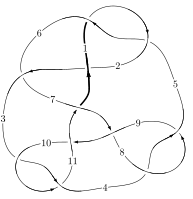
\includegraphics[width=112pt]{../../../GIT/diagram.site/Diagrams/png/349_11a_100.png}\\
\ \ \ A knot diagram\footnotemark}&
\allowdisplaybreaks
\textbf{Linearized knot diagam} \\
\cline{2-2}
 &
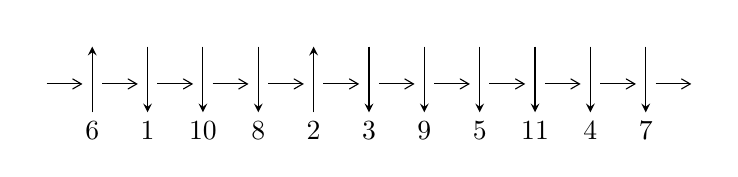
\begin{tikzpicture}[x=20pt, y=17pt]
	% nodes
	\node (C0) at (0, 0) {};
	\node (C1) at (1, 0) {};
	\node (C1U) at (1, +1) {};
	\node (C1D) at (1, -1) {6};

	\node (C2) at (2, 0) {};
	\node (C2U) at (2, +1) {};
	\node (C2D) at (2, -1) {1};

	\node (C3) at (3, 0) {};
	\node (C3U) at (3, +1) {};
	\node (C3D) at (3, -1) {10};

	\node (C4) at (4, 0) {};
	\node (C4U) at (4, +1) {};
	\node (C4D) at (4, -1) {8};

	\node (C5) at (5, 0) {};
	\node (C5U) at (5, +1) {};
	\node (C5D) at (5, -1) {2};

	\node (C6) at (6, 0) {};
	\node (C6U) at (6, +1) {};
	\node (C6D) at (6, -1) {3};

	\node (C7) at (7, 0) {};
	\node (C7U) at (7, +1) {};
	\node (C7D) at (7, -1) {9};

	\node (C8) at (8, 0) {};
	\node (C8U) at (8, +1) {};
	\node (C8D) at (8, -1) {5};

	\node (C9) at (9, 0) {};
	\node (C9U) at (9, +1) {};
	\node (C9D) at (9, -1) {11};

	\node (C10) at (10, 0) {};
	\node (C10U) at (10, +1) {};
	\node (C10D) at (10, -1) {4};

	\node (C11) at (11, 0) {};
	\node (C11U) at (11, +1) {};
	\node (C11D) at (11, -1) {7};
	\node (C12) at (12, 0) {};

	% arrows
	\draw[->,>={angle 60}]
	(C0) edge (C1) (C1) edge (C2) (C2) edge (C3) (C3) edge (C4) (C4) edge (C5) (C5) edge (C6) (C6) edge (C7) (C7) edge (C8) (C8) edge (C9) (C9) edge (C10) (C10) edge (C11) (C11) edge (C12) ;	\draw[->,>=stealth]
	(C1D) edge (C1U) (C2U) edge (C2D) (C3U) edge (C3D) (C4U) edge (C4D) (C5D) edge (C5U) (C6U) edge (C6D) (C7U) edge (C7D) (C8U) edge (C8D) (C9U) edge (C9D) (C10U) edge (C10D) (C11U) edge (C11D) ;
	\end{tikzpicture} \\
\hhline{~~} \\& 
\textbf{Solving Sequence} \\ \cline{2-2} 
 &
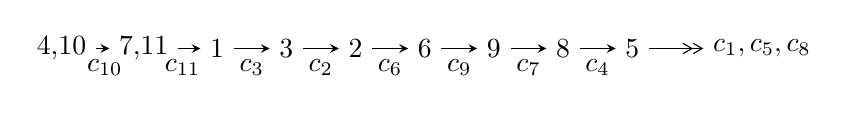
\begin{tikzpicture}[x=25pt, y=7pt]
	% node
	\node (A0) at (-1/8, 0) {4,10};
	\node (A1) at (17/16, 0) {7,11};
	\node (A2) at (17/8, 0) {1};
	\node (A3) at (25/8, 0) {3};
	\node (A4) at (33/8, 0) {2};
	\node (A5) at (41/8, 0) {6};
	\node (A6) at (49/8, 0) {9};
	\node (A7) at (57/8, 0) {8};
	\node (A8) at (65/8, 0) {5};
	\node (C1) at (1/2, -1) {$c_{10}$};
	\node (C2) at (13/8, -1) {$c_{11}$};
	\node (C3) at (21/8, -1) {$c_{3}$};
	\node (C4) at (29/8, -1) {$c_{2}$};
	\node (C5) at (37/8, -1) {$c_{6}$};
	\node (C6) at (45/8, -1) {$c_{9}$};
	\node (C7) at (53/8, -1) {$c_{7}$};
	\node (C8) at (61/8, -1) {$c_{4}$};
	\node (A9) at (10, 0) {$c_{1},c_{5},c_{8}$};

	% edge
	\draw[->,>=stealth]	
	(A0) edge (A1) (A1) edge (A2) (A2) edge (A3) (A3) edge (A4) (A4) edge (A5) (A5) edge (A6) (A6) edge (A7) (A7) edge (A8) ;
	\draw[->>,>={angle 60}]	
	(A8) edge (A9);
\end{tikzpicture} \\ 

\end{tabular} \\

\footnotetext{
The image of knot diagram is generated by the software ``\textbf{Draw programme}" developed by Andrew Bartholomew(\url{http://www.layer8.co.uk/maths/draw/index.htm\#Running-draw}), where we modified some parts for our purpose(\url{https://github.com/CATsTAILs/LinksPainter}).
}\phantom \\ \newline 
\centering \textbf{Ideals for irreducible components\footnotemark of $X_{\text{par}}$} 
 
\begin{align*}
I^u_{1}&=\langle 
u^{30}- u^{29}+\cdots+8 b+u,\;- u^4+u^2+a-1,\;u^{31}- u^{30}+\cdots+2 u-1\rangle \\
I^u_{2}&=\langle 
8.05572\times10^{18} u^{45}-1.78051\times10^{19} u^{44}+\cdots+3.67198\times10^{19} b-7.81561\times10^{18},\\
\phantom{I^u_{2}}&\phantom{= \langle  }9.93809\times10^{19} u^{45}-7.04855\times10^{19} u^{44}+\cdots+3.67198\times10^{19} a-2.19276\times10^{20},\;u^{46}- u^{45}+\cdots-4 u+1\rangle \\
I^u_{3}&=\langle 
b^4+4 b^3+4 b^2+1,\;a+1,\;u+1\rangle \\
I^u_{4}&=\langle 
b^3+3 b^2+3 b+1,\;a+1,\;u-1\rangle \\
\\
\end{align*}
\raggedright * 4 irreducible components of $\dim_{\mathbb{C}}=0$, with total 84 representations.\\
\footnotetext{All coefficients of polynomials are rational numbers. But the coefficients are sometimes approximated in decimal forms when there is not enough margin.}
\newpage
\renewcommand{\arraystretch}{1}
\centering \section*{I. $I^u_{1}= \langle u^{30}- u^{29}+\cdots+8 b+u,\;- u^4+u^2+a-1,\;u^{31}- u^{30}+\cdots+2 u-1 \rangle$}
\flushleft \textbf{(i) Arc colorings}\\
\begin{tabular}{m{7pt} m{180pt} m{7pt} m{180pt} }
\flushright $a_{4}=$&$\begin{pmatrix}0\\u\end{pmatrix}$ \\
\flushright $a_{10}=$&$\begin{pmatrix}1\\0\end{pmatrix}$ \\
\flushright $a_{7}=$&$\begin{pmatrix}u^4- u^2+1\\-\frac{1}{8} u^{30}+\frac{1}{8} u^{29}+\cdots-\frac{3}{4} u^2-\frac{1}{8} u\end{pmatrix}$ \\
\flushright $a_{11}=$&$\begin{pmatrix}1\\u^2\end{pmatrix}$ \\
\flushright $a_{1}=$&$\begin{pmatrix}-\frac{1}{8} u^{30}+\frac{1}{8} u^{29}+\cdots-\frac{1}{8} u+1\\u^{30}-\frac{9}{8} u^{29}+\cdots+\frac{3}{2} u-\frac{1}{8}\end{pmatrix}$ \\
\flushright $a_{3}=$&$\begin{pmatrix}u\\u\end{pmatrix}$ \\
\flushright $a_{2}=$&$\begin{pmatrix}-\frac{1}{2} u^{30}+\frac{1}{8} u^{29}+\cdots+\frac{1}{2} u+\frac{3}{8}\\\frac{13}{8} u^{30}-\frac{27}{8} u^{29}+\cdots+\frac{79}{8} u-3\end{pmatrix}$ \\
\flushright $a_{6}=$&$\begin{pmatrix}-\frac{1}{8} u^{30}+\frac{1}{8} u^{29}+\cdots-\frac{1}{8} u+1\\-\frac{1}{4} u^{30}+\frac{1}{4} u^{29}+\cdots-\frac{3}{2} u^2-\frac{1}{4} u\end{pmatrix}$ \\
\flushright $a_{9}=$&$\begin{pmatrix}- u^2+1\\- u^4\end{pmatrix}$ \\
\flushright $a_{8}=$&$\begin{pmatrix}1\\-\frac{1}{8} u^{30}+\frac{1}{8} u^{29}+\cdots-\frac{3}{4} u^2-\frac{1}{8} u\end{pmatrix}$ \\
\flushright $a_{5}=$&$\begin{pmatrix}- u\\\frac{1}{8} u^{29}-\frac{1}{8} u^{28}+\cdots+\frac{3}{4} u+\frac{1}{8}\end{pmatrix}$\\ \flushright $a_{5}=$&$\begin{pmatrix}- u\\\frac{1}{8} u^{29}-\frac{1}{8} u^{28}+\cdots+\frac{3}{4} u+\frac{1}{8}\end{pmatrix}$\\&\end{tabular}
\flushleft \textbf{(ii) Obstruction class $= -1$}\\~\\
\flushleft \textbf{(iii) Cusp Shapes $= \frac{3}{2} u^{30}-\frac{17}{4} u^{29}+\cdots+\frac{49}{2} u-\frac{69}{4}$}\\~\\
\newpage\renewcommand{\arraystretch}{1}
\flushleft \textbf{(iv) u-Polynomials at the component}\newline \\
\begin{tabular}{m{50pt}|m{274pt}}
Crossings & \hspace{64pt}u-Polynomials at each crossing \\
\hline $$\begin{aligned}c_{1},c_{5}\end{aligned}$$&$\begin{aligned}
&u^{31}-3 u^{30}+\cdots-6 u+2
\end{aligned}$\\
\hline $$\begin{aligned}c_{2}\end{aligned}$$&$\begin{aligned}
&u^{31}+15 u^{30}+\cdots-4 u-4
\end{aligned}$\\
\hline $$\begin{aligned}c_{3},c_{4},c_{8}\\c_{10}\end{aligned}$$&$\begin{aligned}
&u^{31}+u^{30}+\cdots+2 u+1
\end{aligned}$\\
\hline $$\begin{aligned}c_{6}\end{aligned}$$&$\begin{aligned}
&u^{31}+3 u^{30}+\cdots+34 u+2
\end{aligned}$\\
\hline $$\begin{aligned}c_{7},c_{9}\end{aligned}$$&$\begin{aligned}
&u^{31}+13 u^{30}+\cdots+8 u+1
\end{aligned}$\\
\hline $$\begin{aligned}c_{11}\end{aligned}$$&$\begin{aligned}
&u^{31}-15 u^{30}+\cdots-1566 u+158
\end{aligned}$\\
\hline
\end{tabular}\\~\\
\newpage\renewcommand{\arraystretch}{1}
\flushleft \textbf{(v) Riley Polynomials at the component}\newline \\
\begin{tabular}{m{50pt}|m{274pt}}
Crossings & \hspace{64pt}Riley Polynomials at each crossing \\
\hline $$\begin{aligned}c_{1},c_{5}\end{aligned}$$&$\begin{aligned}
&y^{31}+15 y^{30}+\cdots-4 y-4
\end{aligned}$\\
\hline $$\begin{aligned}c_{2}\end{aligned}$$&$\begin{aligned}
&y^{31}+3 y^{30}+\cdots+112 y-16
\end{aligned}$\\
\hline $$\begin{aligned}c_{3},c_{4},c_{8}\\c_{10}\end{aligned}$$&$\begin{aligned}
&y^{31}-13 y^{30}+\cdots+8 y-1
\end{aligned}$\\
\hline $$\begin{aligned}c_{6}\end{aligned}$$&$\begin{aligned}
&y^{31}-9 y^{30}+\cdots+92 y-4
\end{aligned}$\\
\hline $$\begin{aligned}c_{7},c_{9}\end{aligned}$$&$\begin{aligned}
&y^{31}+19 y^{30}+\cdots-4 y-1
\end{aligned}$\\
\hline $$\begin{aligned}c_{11}\end{aligned}$$&$\begin{aligned}
&y^{31}+3 y^{30}+\cdots-219108 y-24964
\end{aligned}$\\
\hline
\end{tabular}\\~\\
\newpage\flushleft \textbf{(vi) Complex Volumes and Cusp Shapes}
$$\begin{array}{c|c|c}  
\text{Solutions to }I^u_{1}& \I (\text{vol} + \sqrt{-1}CS) & \text{Cusp shape}\\
 \hline 
\begin{aligned}
u &= -0.671875 + 0.755704 I \\
a &= \phantom{-}0.102801 + 1.258530 I \\
b &= \phantom{-}1.26875 + 0.87692 I\end{aligned}
 & \phantom{-}4.33630 + 2.18000 I & -1.38223 - 2.85674 I \\ \hline\begin{aligned}
u &= -0.671875 - 0.755704 I \\
a &= \phantom{-}0.102801 - 1.258530 I \\
b &= \phantom{-}1.26875 - 0.87692 I\end{aligned}
 & \phantom{-}4.33630 - 2.18000 I & -1.38223 + 2.85674 I \\ \hline\begin{aligned}
u &= -0.529243 + 0.781629 I \\
a &= \phantom{-}0.75581 + 1.37479 I \\
b &= \phantom{-}1.228420 + 0.141119 I\end{aligned}
 & \phantom{-}3.92659 - 0.20488 I & -1.21175 - 1.93479 I \\ \hline\begin{aligned}
u &= -0.529243 - 0.781629 I \\
a &= \phantom{-}0.75581 - 1.37479 I \\
b &= \phantom{-}1.228420 - 0.141119 I\end{aligned}
 & \phantom{-}3.92659 + 0.20488 I & -1.21175 + 1.93479 I \\ \hline\begin{aligned}
u &= \phantom{-}0.473734 + 0.815861 I \\
a &= \phantom{-}1.03834 - 1.45511 I \\
b &= \phantom{-}1.186120 + 0.184502 I\end{aligned}
 & \phantom{-}1.98591 + 5.18766 I & -4.29263 - 2.87164 I \\ \hline\begin{aligned}
u &= \phantom{-}0.473734 - 0.815861 I \\
a &= \phantom{-}1.03834 + 1.45511 I \\
b &= \phantom{-}1.186120 - 0.184502 I\end{aligned}
 & \phantom{-}1.98591 - 5.18766 I & -4.29263 + 2.87164 I \\ \hline\begin{aligned}
u &= \phantom{-}0.739148 + 0.756876 I \\
a &= -0.224684 - 1.178240 I \\
b &= \phantom{-}1.18263 - 1.25006 I\end{aligned}
 & \phantom{-}2.80358 - 7.15169 I & -4.41360 + 8.13736 I \\ \hline\begin{aligned}
u &= \phantom{-}0.739148 - 0.756876 I \\
a &= -0.224684 + 1.178240 I \\
b &= \phantom{-}1.18263 + 1.25006 I\end{aligned}
 & \phantom{-}2.80358 + 7.15169 I & -4.41360 - 8.13736 I \\ \hline\begin{aligned}
u &= -0.998773 + 0.420018 I \\
a &= \phantom{-}0.149196 - 0.538864 I \\
b &= \phantom{-}1.154630 + 0.334617 I\end{aligned}
 & -5.71846 - 1.00535 I & -12.20049 - 2.17594 I \\ \hline\begin{aligned}
u &= -0.998773 - 0.420018 I \\
a &= \phantom{-}0.149196 + 0.538864 I \\
b &= \phantom{-}1.154630 - 0.334617 I\end{aligned}
 & -5.71846 + 1.00535 I & -12.20049 + 2.17594 I\\
 \hline 
 \end{array}$$\newpage$$\begin{array}{c|c|c}  
\text{Solutions to }I^u_{1}& \I (\text{vol} + \sqrt{-1}CS) & \text{Cusp shape}\\
 \hline 
\begin{aligned}
u &= \phantom{-}1.001180 + 0.470735 I \\
a &= -0.059625 + 0.529287 I \\
b &= \phantom{-}0.707502 - 0.184028 I\end{aligned}
 & -2.76836 - 3.54859 I & -8.60512 + 5.21629 I \\ \hline\begin{aligned}
u &= \phantom{-}1.001180 - 0.470735 I \\
a &= -0.059625 - 0.529287 I \\
b &= \phantom{-}0.707502 + 0.184028 I\end{aligned}
 & -2.76836 + 3.54859 I & -8.60512 - 5.21629 I \\ \hline\begin{aligned}
u &= -1.060830 + 0.466616 I \\
a &= -0.063939 - 0.807099 I \\
b &= \phantom{-}0.799755 - 0.463575 I\end{aligned}
 & -6.59629 + 7.25038 I & -13.7743 - 8.1656 I \\ \hline\begin{aligned}
u &= -1.060830 - 0.466616 I \\
a &= -0.063939 + 0.807099 I \\
b &= \phantom{-}0.799755 + 0.463575 I\end{aligned}
 & -6.59629 - 7.25038 I & -13.7743 + 8.1656 I \\ \hline\begin{aligned}
u &= \phantom{-}1.045460 + 0.641230 I \\
a &= -1.014590 + 0.487534 I \\
b &= -1.013330 - 0.611771 I\end{aligned}
 & \phantom{-}0.83772 - 3.66094 I & -6.42863 + 2.29820 I \\ \hline\begin{aligned}
u &= \phantom{-}1.045460 - 0.641230 I \\
a &= -1.014590 - 0.487534 I \\
b &= -1.013330 + 0.611771 I\end{aligned}
 & \phantom{-}0.83772 + 3.66094 I & -6.42863 - 2.29820 I \\ \hline\begin{aligned}
u &= \phantom{-}0.551309 + 0.517564 I \\
a &= \phantom{-}0.639561 - 0.529508 I \\
b &= \phantom{-}0.464527 - 0.522513 I\end{aligned}
 & -0.67493 - 1.41882 I & -8.11819 + 4.23209 I \\ \hline\begin{aligned}
u &= \phantom{-}0.551309 - 0.517564 I \\
a &= \phantom{-}0.639561 + 0.529508 I \\
b &= \phantom{-}0.464527 + 0.522513 I\end{aligned}
 & -0.67493 + 1.41882 I & -8.11819 - 4.23209 I \\ \hline\begin{aligned}
u &= -1.093950 + 0.638128 I \\
a &= -1.115430 - 0.808402 I \\
b &= -1.54639 + 0.11518 I\end{aligned}
 & \phantom{-}1.61779 + 8.62066 I & -5.39345 - 7.96064 I \\ \hline\begin{aligned}
u &= -1.093950 - 0.638128 I \\
a &= -1.115430 + 0.808402 I \\
b &= -1.54639 - 0.11518 I\end{aligned}
 & \phantom{-}1.61779 - 8.62066 I & -5.39345 + 7.96064 I\\
 \hline 
 \end{array}$$\newpage$$\begin{array}{c|c|c}  
\text{Solutions to }I^u_{1}& \I (\text{vol} + \sqrt{-1}CS) & \text{Cusp shape}\\
 \hline 
\begin{aligned}
u &= \phantom{-}1.150290 + 0.579146 I \\
a &= -0.78731 + 1.29973 I \\
b &= -1.32274 + 1.36596 I\end{aligned}
 & -4.83518 - 8.17855 I & -13.0634 + 5.6311 I \\ \hline\begin{aligned}
u &= \phantom{-}1.150290 - 0.579146 I \\
a &= -0.78731 - 1.29973 I \\
b &= -1.32274 - 1.36596 I\end{aligned}
 & -4.83518 + 8.17855 I & -13.0634 - 5.6311 I \\ \hline\begin{aligned}
u &= -1.159090 + 0.618451 I \\
a &= -1.09291 - 1.32186 I \\
b &= -2.11523 - 1.06499 I\end{aligned}
 & -0.06269 + 11.03950 I & -6.94221 - 7.13356 I \\ \hline\begin{aligned}
u &= -1.159090 - 0.618451 I \\
a &= -1.09291 + 1.32186 I \\
b &= -2.11523 + 1.06499 I\end{aligned}
 & -0.06269 - 11.03950 I & -6.94221 + 7.13356 I \\ \hline\begin{aligned}
u &= -0.673147 + 0.057260 I \\
a &= \phantom{-}0.746573 + 0.007732 I \\
b &= -1.032490 + 0.376155 I\end{aligned}
 & -4.34804 + 3.91818 I & -8.50345 - 5.07903 I \\ \hline\begin{aligned}
u &= -0.673147 - 0.057260 I \\
a &= \phantom{-}0.746573 - 0.007732 I \\
b &= -1.032490 - 0.376155 I\end{aligned}
 & -4.34804 - 3.91818 I & -8.50345 + 5.07903 I \\ \hline\begin{aligned}
u &= \phantom{-}1.179340 + 0.616871 I \\
a &= -1.10660 + 1.48500 I \\
b &= -2.36523 + 1.45569 I\end{aligned}
 & -2.4315 - 16.1755 I & -10.0749 + 10.7687 I \\ \hline\begin{aligned}
u &= \phantom{-}1.179340 - 0.616871 I \\
a &= -1.10660 - 1.48500 I \\
b &= -2.36523 - 1.45569 I\end{aligned}
 & -2.4315 + 16.1755 I & -10.0749 - 10.7687 I \\ \hline\begin{aligned}
u &= \phantom{-}0.581693\phantom{ +0.000000I} \\
a &= \phantom{-}0.776125\phantom{ +0.000000I} \\
b &= -0.645714\phantom{ +0.000000I}\end{aligned}
 & -1.33697\phantom{ +0.000000I} & -6.39560\phantom{ +0.000000I} \\ \hline\begin{aligned}
u &= \phantom{-}0.255598 + 0.492030 I \\
a &= \phantom{-}1.144740 - 0.340444 I \\
b &= \phantom{-}0.225939 - 0.088212 I\end{aligned}
 & -0.56339 - 1.34523 I & -5.39791 + 4.30982 I\\
 \hline 
 \end{array}$$\newpage$$\begin{array}{c|c|c}  
\text{Solutions to }I^u_{1}& \I (\text{vol} + \sqrt{-1}CS) & \text{Cusp shape}\\
 \hline 
\begin{aligned}
u &= \phantom{-}0.255598 - 0.492030 I \\
a &= \phantom{-}1.144740 + 0.340444 I \\
b &= \phantom{-}0.225939 + 0.088212 I\end{aligned}
 & -0.56339 + 1.34523 I & -5.39791 - 4.30982 I\\
 \hline 
 \end{array}$$\newpage\newpage\renewcommand{\arraystretch}{1}
\centering \section*{II. $I^u_{2}= \langle 8.06\times10^{18} u^{45}-1.78\times10^{19} u^{44}+\cdots+3.67\times10^{19} b-7.82\times10^{18},\;9.94\times10^{19} u^{45}-7.05\times10^{19} u^{44}+\cdots+3.67\times10^{19} a-2.19\times10^{20},\;u^{46}- u^{45}+\cdots-4 u+1 \rangle$}
\flushleft \textbf{(i) Arc colorings}\\
\begin{tabular}{m{7pt} m{180pt} m{7pt} m{180pt} }
\flushright $a_{4}=$&$\begin{pmatrix}0\\u\end{pmatrix}$ \\
\flushright $a_{10}=$&$\begin{pmatrix}1\\0\end{pmatrix}$ \\
\flushright $a_{7}=$&$\begin{pmatrix}-2.70647 u^{45}+1.91955 u^{44}+\cdots-10.9263 u+5.97160\\-0.219384 u^{45}+0.484891 u^{44}+\cdots-1.60887 u+0.212845\end{pmatrix}$ \\
\flushright $a_{11}=$&$\begin{pmatrix}1\\u^2\end{pmatrix}$ \\
\flushright $a_{1}=$&$\begin{pmatrix}3.33142 u^{45}-2.00063 u^{44}+\cdots+10.3559 u-4.02342\\1.22417 u^{45}-1.02774 u^{44}+\cdots+3.03021 u-0.595457\end{pmatrix}$ \\
\flushright $a_{3}=$&$\begin{pmatrix}u\\u\end{pmatrix}$ \\
\flushright $a_{2}=$&$\begin{pmatrix}4.37249 u^{45}-1.83378 u^{44}+\cdots+15.1410 u-3.15401\\2.88125 u^{45}-1.87484 u^{44}+\cdots+10.2725 u-3.36688\end{pmatrix}$ \\
\flushright $a_{6}=$&$\begin{pmatrix}-3.03496 u^{45}+2.13094 u^{44}+\cdots-9.20367 u+4.91918\\-0.547882 u^{45}+0.696284 u^{44}+\cdots+0.113735 u-0.839578\end{pmatrix}$ \\
\flushright $a_{9}=$&$\begin{pmatrix}- u^2+1\\- u^4\end{pmatrix}$ \\
\flushright $a_{8}=$&$\begin{pmatrix}-2.33885 u^{45}+1.49981 u^{44}+\cdots-8.74130 u+5.70663\\0.536038 u^{45}-0.110109 u^{44}+\cdots-1.01730 u-0.160962\end{pmatrix}$ \\
\flushright $a_{5}=$&$\begin{pmatrix}0.160962 u^{45}+0.375077 u^{44}+\cdots+3.35122 u-1.66115\\-0.413110 u^{45}+1.85280 u^{44}+\cdots-0.665590 u+1.80281\end{pmatrix}$\\ \flushright $a_{5}=$&$\begin{pmatrix}0.160962 u^{45}+0.375077 u^{44}+\cdots+3.35122 u-1.66115\\-0.413110 u^{45}+1.85280 u^{44}+\cdots-0.665590 u+1.80281\end{pmatrix}$\\&\end{tabular}
\flushleft \textbf{(ii) Obstruction class $= -1$}\\~\\
\flushleft \textbf{(iii) Cusp Shapes $= -\frac{13372946836041823816}{36719786468444867913} u^{45}+\frac{53663175405029739464}{36719786468444867913} u^{44}+\cdots+\frac{374972108042035142776}{36719786468444867913} u-\frac{316536124285645900534}{36719786468444867913}$}\\~\\
\newpage\renewcommand{\arraystretch}{1}
\flushleft \textbf{(iv) u-Polynomials at the component}\newline \\
\begin{tabular}{m{50pt}|m{274pt}}
Crossings & \hspace{64pt}u-Polynomials at each crossing \\
\hline $$\begin{aligned}c_{1},c_{5}\end{aligned}$$&$\begin{aligned}
&(u^{23}+u^{22}+\cdots+2 u+1)^{2}
\end{aligned}$\\
\hline $$\begin{aligned}c_{2}\end{aligned}$$&$\begin{aligned}
&(u^{23}+11 u^{22}+\cdots-2 u^2-1)^{2}
\end{aligned}$\\
\hline $$\begin{aligned}c_{3},c_{4},c_{8}\\c_{10}\end{aligned}$$&$\begin{aligned}
&u^{46}+u^{45}+\cdots+4 u+1
\end{aligned}$\\
\hline $$\begin{aligned}c_{6}\end{aligned}$$&$\begin{aligned}
&(u^{23}- u^{22}+\cdots-8 u+5)^{2}
\end{aligned}$\\
\hline $$\begin{aligned}c_{7},c_{9}\end{aligned}$$&$\begin{aligned}
&u^{46}+25 u^{45}+\cdots+4 u+1
\end{aligned}$\\
\hline $$\begin{aligned}c_{11}\end{aligned}$$&$\begin{aligned}
&(u^{23}+5 u^{22}+\cdots+32 u+7)^{2}
\end{aligned}$\\
\hline
\end{tabular}\\~\\
\newpage\renewcommand{\arraystretch}{1}
\flushleft \textbf{(v) Riley Polynomials at the component}\newline \\
\begin{tabular}{m{50pt}|m{274pt}}
Crossings & \hspace{64pt}Riley Polynomials at each crossing \\
\hline $$\begin{aligned}c_{1},c_{5}\end{aligned}$$&$\begin{aligned}
&(y^{23}+11 y^{22}+\cdots-2 y^2-1)^{2}
\end{aligned}$\\
\hline $$\begin{aligned}c_{2}\end{aligned}$$&$\begin{aligned}
&(y^{23}+3 y^{22}+\cdots-4 y-1)^{2}
\end{aligned}$\\
\hline $$\begin{aligned}c_{3},c_{4},c_{8}\\c_{10}\end{aligned}$$&$\begin{aligned}
&y^{46}-25 y^{45}+\cdots-4 y+1
\end{aligned}$\\
\hline $$\begin{aligned}c_{6}\end{aligned}$$&$\begin{aligned}
&(y^{23}-5 y^{22}+\cdots+264 y-25)^{2}
\end{aligned}$\\
\hline $$\begin{aligned}c_{7},c_{9}\end{aligned}$$&$\begin{aligned}
&y^{46}-9 y^{45}+\cdots-104 y+1
\end{aligned}$\\
\hline $$\begin{aligned}c_{11}\end{aligned}$$&$\begin{aligned}
&(y^{23}+7 y^{22}+\cdots-404 y-49)^{2}
\end{aligned}$\\
\hline
\end{tabular}\\~\\
\newpage\flushleft \textbf{(vi) Complex Volumes and Cusp Shapes}
$$\begin{array}{c|c|c}  
\text{Solutions to }I^u_{2}& \I (\text{vol} + \sqrt{-1}CS) & \text{Cusp shape}\\
 \hline 
\begin{aligned}
u &= \phantom{-}0.326451 + 0.907420 I \\
a &= -0.77255 + 1.54332 I \\
b &= -1.111200 - 0.111182 I\end{aligned}
 & \phantom{-}0.14155 + 10.59580 I & -6.96908 - 7.47788 I \\ \hline\begin{aligned}
u &= \phantom{-}0.326451 - 0.907420 I \\
a &= -0.77255 - 1.54332 I \\
b &= -1.111200 + 0.111182 I\end{aligned}
 & \phantom{-}0.14155 - 10.59580 I & -6.96908 + 7.47788 I \\ \hline\begin{aligned}
u &= \phantom{-}0.539847 + 0.797694 I \\
a &= \phantom{-}0.530178 + 0.740332 I \\
b &= -0.897400 + 0.896177 I\end{aligned}
 & \phantom{-}2.35134 - 1.73636 I & -4.20687 + 2.46590 I \\ \hline\begin{aligned}
u &= \phantom{-}0.539847 - 0.797694 I \\
a &= \phantom{-}0.530178 - 0.740332 I \\
b &= -0.897400 - 0.896177 I\end{aligned}
 & \phantom{-}2.35134 + 1.73636 I & -4.20687 - 2.46590 I \\ \hline\begin{aligned}
u &= -0.466971 + 0.825572 I \\
a &= \phantom{-}0.159069 - 0.983222 I \\
b &= -1.088190 - 0.614230 I\end{aligned}
 & \phantom{-}3.49101 - 3.16234 I & -2.33540 + 3.46689 I \\ \hline\begin{aligned}
u &= -0.466971 - 0.825572 I \\
a &= \phantom{-}0.159069 + 0.983222 I \\
b &= -1.088190 + 0.614230 I\end{aligned}
 & \phantom{-}3.49101 + 3.16234 I & -2.33540 - 3.46689 I \\ \hline\begin{aligned}
u &= -0.356156 + 0.878751 I \\
a &= -0.54445 - 1.35389 I \\
b &= -1.126660 - 0.091255 I\end{aligned}
 & \phantom{-}2.34965 - 5.52406 I & -3.72778 + 3.52157 I \\ \hline\begin{aligned}
u &= -0.356156 - 0.878751 I \\
a &= -0.54445 + 1.35389 I \\
b &= -1.126660 + 0.091255 I\end{aligned}
 & \phantom{-}2.34965 + 5.52406 I & -3.72778 - 3.52157 I \\ \hline\begin{aligned}
u &= -1.036260 + 0.200630 I \\
a &= -0.031632 + 0.423510 I \\
b &= -0.996138 + 0.538101 I\end{aligned}
 & -4.31524 + 3.60580 I & -10.88555 - 4.48858 I \\ \hline\begin{aligned}
u &= -1.036260 - 0.200630 I \\
a &= -0.031632 - 0.423510 I \\
b &= -0.996138 - 0.538101 I\end{aligned}
 & -4.31524 - 3.60580 I & -10.88555 + 4.48858 I\\
 \hline 
 \end{array}$$\newpage$$\begin{array}{c|c|c}  
\text{Solutions to }I^u_{2}& \I (\text{vol} + \sqrt{-1}CS) & \text{Cusp shape}\\
 \hline 
\begin{aligned}
u &= -0.976746 + 0.435286 I \\
a &= -0.94989 - 2.08219 I \\
b &= -1.89184 - 1.72781 I\end{aligned}
 & -3.06946 + 2.29224 I & -8.17333 - 3.81893 I \\ \hline\begin{aligned}
u &= -0.976746 - 0.435286 I \\
a &= -0.94989 + 2.08219 I \\
b &= -1.89184 + 1.72781 I\end{aligned}
 & -3.06946 - 2.29224 I & -8.17333 + 3.81893 I \\ \hline\begin{aligned}
u &= \phantom{-}0.886233 + 0.678199 I \\
a &= \phantom{-}1.217710 - 0.695264 I \\
b &= \phantom{-}1.155150 + 0.542637 I\end{aligned}
 & \phantom{-}2.35134 + 1.73636 I & -4.20687 - 2.46590 I \\ \hline\begin{aligned}
u &= \phantom{-}0.886233 - 0.678199 I \\
a &= \phantom{-}1.217710 + 0.695264 I \\
b &= \phantom{-}1.155150 - 0.542637 I\end{aligned}
 & \phantom{-}2.35134 - 1.73636 I & -4.20687 + 2.46590 I \\ \hline\begin{aligned}
u &= \phantom{-}1.009630 + 0.482481 I \\
a &= -0.74786 + 2.38510 I \\
b &= -2.07366 + 2.28227 I\end{aligned}
 & -5.29128 - 7.02777 I & -11.56401 + 7.34039 I \\ \hline\begin{aligned}
u &= \phantom{-}1.009630 - 0.482481 I \\
a &= -0.74786 - 2.38510 I \\
b &= -2.07366 - 2.28227 I\end{aligned}
 & -5.29128 + 7.02777 I & -11.56401 - 7.34039 I \\ \hline\begin{aligned}
u &= -0.807547 + 0.331658 I \\
a &= -1.81318 - 1.49133 I \\
b &= -1.88066 - 0.51355 I\end{aligned}
 & -2.27583 + 0.94673 I & -5.56367 - 4.33310 I \\ \hline\begin{aligned}
u &= -0.807547 - 0.331658 I \\
a &= -1.81318 + 1.49133 I \\
b &= -1.88066 + 0.51355 I\end{aligned}
 & -2.27583 - 0.94673 I & -5.56367 + 4.33310 I \\ \hline\begin{aligned}
u &= \phantom{-}0.296950 + 0.801445 I \\
a &= -0.872198 + 0.800219 I \\
b &= -0.792177 + 0.162915 I\end{aligned}
 & -2.33291 + 3.02476 I & -10.12213 - 2.21609 I \\ \hline\begin{aligned}
u &= \phantom{-}0.296950 - 0.801445 I \\
a &= -0.872198 - 0.800219 I \\
b &= -0.792177 - 0.162915 I\end{aligned}
 & -2.33291 - 3.02476 I & -10.12213 + 2.21609 I\\
 \hline 
 \end{array}$$\newpage$$\begin{array}{c|c|c}  
\text{Solutions to }I^u_{2}& \I (\text{vol} + \sqrt{-1}CS) & \text{Cusp shape}\\
 \hline 
\begin{aligned}
u &= \phantom{-}1.079890 + 0.398169 I \\
a &= -0.33037 + 1.80790 I \\
b &= -0.88071 + 2.08789 I\end{aligned}
 & -7.03235 + 0.30335 I & -15.4115 + 0.4048 I \\ \hline\begin{aligned}
u &= \phantom{-}1.079890 - 0.398169 I \\
a &= -0.33037 - 1.80790 I \\
b &= -0.88071 - 2.08789 I\end{aligned}
 & -7.03235 - 0.30335 I & -15.4115 - 0.4048 I \\ \hline\begin{aligned}
u &= -0.952704 + 0.656540 I \\
a &= \phantom{-}1.13459 + 0.99283 I \\
b &= \phantom{-}1.52639 + 0.00115 I\end{aligned}
 & \phantom{-}3.49101 + 3.16234 I & -2.33540 - 3.46689 I \\ \hline\begin{aligned}
u &= -0.952704 - 0.656540 I \\
a &= \phantom{-}1.13459 - 0.99283 I \\
b &= \phantom{-}1.52639 - 0.00115 I\end{aligned}
 & \phantom{-}3.49101 - 3.16234 I & -2.33540 + 3.46689 I \\ \hline\begin{aligned}
u &= \phantom{-}1.050590 + 0.549581 I \\
a &= \phantom{-}0.568130 - 1.260550 I \\
b &= \phantom{-}1.01651 - 1.37602 I\end{aligned}
 & -2.33291 - 3.02476 I & -10.12213 + 2.21609 I \\ \hline\begin{aligned}
u &= \phantom{-}1.050590 - 0.549581 I \\
a &= \phantom{-}0.568130 + 1.260550 I \\
b &= \phantom{-}1.01651 + 1.37602 I\end{aligned}
 & -2.33291 + 3.02476 I & -10.12213 - 2.21609 I \\ \hline\begin{aligned}
u &= \phantom{-}1.213100 + 0.082369 I \\
a &= -0.285118 + 0.176496 I \\
b &= -0.551742 - 0.474744 I\end{aligned}
 & -2.27583 + 0.94673 I & -5.56367 - 4.33310 I \\ \hline\begin{aligned}
u &= \phantom{-}1.213100 - 0.082369 I \\
a &= -0.285118 - 0.176496 I \\
b &= -0.551742 + 0.474744 I\end{aligned}
 & -2.27583 - 0.94673 I & -5.56367 + 4.33310 I \\ \hline\begin{aligned}
u &= -1.219100 + 0.005734 I \\
a &= -0.379506 + 0.077327 I \\
b &= -1.217710 - 0.486619 I\end{aligned}
 & -3.90982 - 3.26242 I & -8.80376 + 2.26815 I \\ \hline\begin{aligned}
u &= -1.219100 - 0.005734 I \\
a &= -0.379506 - 0.077327 I \\
b &= -1.217710 + 0.486619 I\end{aligned}
 & -3.90982 + 3.26242 I & -8.80376 - 2.26815 I\\
 \hline 
 \end{array}$$\newpage$$\begin{array}{c|c|c}  
\text{Solutions to }I^u_{2}& \I (\text{vol} + \sqrt{-1}CS) & \text{Cusp shape}\\
 \hline 
\begin{aligned}
u &= -1.054910 + 0.629750 I \\
a &= \phantom{-}0.89707 + 1.44259 I \\
b &= \phantom{-}1.92867 + 1.14714 I\end{aligned}
 & \phantom{-}2.34965 + 5.52406 I & -3.72778 - 3.52157 I \\ \hline\begin{aligned}
u &= -1.054910 - 0.629750 I \\
a &= \phantom{-}0.89707 - 1.44259 I \\
b &= \phantom{-}1.92867 - 1.14714 I\end{aligned}
 & \phantom{-}2.34965 - 5.52406 I & -3.72778 + 3.52157 I \\ \hline\begin{aligned}
u &= -1.223310 + 0.272825 I \\
a &= \phantom{-}0.227490 - 0.807258 I \\
b &= \phantom{-}0.791557 - 0.749493 I\end{aligned}
 & -7.03235 + 0.30335 I & -15.4115 + 0. I\phantom{ +0.000000I} \\ \hline\begin{aligned}
u &= -1.223310 - 0.272825 I \\
a &= \phantom{-}0.227490 + 0.807258 I \\
b &= \phantom{-}0.791557 + 0.749493 I\end{aligned}
 & -7.03235 - 0.30335 I & -15.4115 + 0. I\phantom{ +0.000000I} \\ \hline\begin{aligned}
u &= \phantom{-}1.089410 + 0.631074 I \\
a &= \phantom{-}0.82929 - 1.61402 I \\
b &= \phantom{-}2.12255 - 1.58531 I\end{aligned}
 & \phantom{-}0.14155 - 10.59580 I & -7.00000 + 7.47788 I \\ \hline\begin{aligned}
u &= \phantom{-}1.089410 - 0.631074 I \\
a &= \phantom{-}0.82929 + 1.61402 I \\
b &= \phantom{-}2.12255 + 1.58531 I\end{aligned}
 & \phantom{-}0.14155 + 10.59580 I & -7.00000 - 7.47788 I \\ \hline\begin{aligned}
u &= \phantom{-}1.260980 + 0.195080 I \\
a &= \phantom{-}0.136063 + 0.360918 I \\
b &= \phantom{-}0.638559 - 0.316478 I\end{aligned}
 & -3.06946 + 2.29224 I & -7.00000 - 3.81893 I \\ \hline\begin{aligned}
u &= \phantom{-}1.260980 - 0.195080 I \\
a &= \phantom{-}0.136063 - 0.360918 I \\
b &= \phantom{-}0.638559 + 0.316478 I\end{aligned}
 & -3.06946 - 2.29224 I & -7.00000 + 3.81893 I \\ \hline\begin{aligned}
u &= -1.294740 + 0.221264 I \\
a &= \phantom{-}0.355915 - 0.330975 I \\
b &= \phantom{-}1.227850 + 0.392277 I\end{aligned}
 & -5.29128 - 7.02777 I & -11.56401 + 7.34039 I \\ \hline\begin{aligned}
u &= -1.294740 - 0.221264 I \\
a &= \phantom{-}0.355915 + 0.330975 I \\
b &= \phantom{-}1.227850 - 0.392277 I\end{aligned}
 & -5.29128 + 7.02777 I & -11.56401 - 7.34039 I\\
 \hline 
 \end{array}$$\newpage$$\begin{array}{c|c|c}  
\text{Solutions to }I^u_{2}& \I (\text{vol} + \sqrt{-1}CS) & \text{Cusp shape}\\
 \hline 
\begin{aligned}
u &= \phantom{-}0.594081 + 0.341794 I \\
a &= -2.68688 + 1.47263 I \\
b &= -1.88722 - 0.13661 I\end{aligned}
 & -3.90982 + 3.26242 I & -8.80376 - 2.26815 I \\ \hline\begin{aligned}
u &= \phantom{-}0.594081 - 0.341794 I \\
a &= -2.68688 - 1.47263 I \\
b &= -1.88722 + 0.13661 I\end{aligned}
 & -3.90982 - 3.26242 I & -8.80376 + 2.26815 I \\ \hline\begin{aligned}
u &= \phantom{-}0.663527\phantom{ +0.000000I} \\
a &= \phantom{-}0.600867\phantom{ +0.000000I} \\
b &= -0.631190\phantom{ +0.000000I}\end{aligned}
 & -1.33670\phantom{ +0.000000I} & -6.47390\phantom{ +0.000000I} \\ \hline\begin{aligned}
u &= \phantom{-}0.486649\phantom{ +0.000000I} \\
a &= \phantom{-}1.02746\phantom{ +0.000000I} \\
b &= -0.652402\phantom{ +0.000000I}\end{aligned}
 & -1.33670\phantom{ +0.000000I} & -6.47390\phantom{ +0.000000I} \\ \hline\begin{aligned}
u &= -0.033796 + 0.382833 I \\
a &= -1.45604 + 2.22878 I \\
b &= -0.870135 - 0.373642 I\end{aligned}
 & -4.31524 - 3.60580 I & -10.88555 + 4.48858 I \\ \hline\begin{aligned}
u &= -0.033796 - 0.382833 I \\
a &= -1.45604 - 2.22878 I \\
b &= -0.870135 + 0.373642 I\end{aligned}
 & -4.31524 + 3.60580 I & -10.88555 - 4.48858 I\\
 \hline 
 \end{array}$$\newpage\newpage\renewcommand{\arraystretch}{1}
\centering \section*{III. $I^u_{3}= \langle b^4+4 b^3+4 b^2+1,\;a+1,\;u+1 \rangle$}
\flushleft \textbf{(i) Arc colorings}\\
\begin{tabular}{m{7pt} m{180pt} m{7pt} m{180pt} }
\flushright $a_{4}=$&$\begin{pmatrix}0\\-1\end{pmatrix}$ \\
\flushright $a_{10}=$&$\begin{pmatrix}1\\0\end{pmatrix}$ \\
\flushright $a_{7}=$&$\begin{pmatrix}-1\\b\end{pmatrix}$ \\
\flushright $a_{11}=$&$\begin{pmatrix}1\\1\end{pmatrix}$ \\
\flushright $a_{1}=$&$\begin{pmatrix}- b\\b^2+b+1\end{pmatrix}$ \\
\flushright $a_{3}=$&$\begin{pmatrix}-1\\-1\end{pmatrix}$ \\
\flushright $a_{2}=$&$\begin{pmatrix}- b^3-2 b^2- b-1\\- b^3+3 b-1\end{pmatrix}$ \\
\flushright $a_{6}=$&$\begin{pmatrix}b\\2 b+1\end{pmatrix}$ \\
\flushright $a_{9}=$&$\begin{pmatrix}0\\-1\end{pmatrix}$ \\
\flushright $a_{8}=$&$\begin{pmatrix}-1\\b-1\end{pmatrix}$ \\
\flushright $a_{5}=$&$\begin{pmatrix}1\\- b\end{pmatrix}$\\ \flushright $a_{5}=$&$\begin{pmatrix}1\\- b\end{pmatrix}$\\&\end{tabular}
\flushleft \textbf{(ii) Obstruction class $= 1$}\\~\\
\flushleft \textbf{(iii) Cusp Shapes $= 4 b^2+8 b-16$}\\~\\
\newpage\renewcommand{\arraystretch}{1}
\flushleft \textbf{(iv) u-Polynomials at the component}\newline \\
\begin{tabular}{m{50pt}|m{274pt}}
Crossings & \hspace{64pt}u-Polynomials at each crossing \\
\hline $$\begin{aligned}c_{1},c_{5}\end{aligned}$$&$\begin{aligned}
&u^4+2 u^2+2
\end{aligned}$\\
\hline $$\begin{aligned}c_{2}\end{aligned}$$&$\begin{aligned}
&(u^2+2 u+2)^2
\end{aligned}$\\
\hline $$\begin{aligned}c_{3},c_{7},c_{8}\\c_{9}\end{aligned}$$&$\begin{aligned}
&(u-1)^4
\end{aligned}$\\
\hline $$\begin{aligned}c_{4},c_{10}\end{aligned}$$&$\begin{aligned}
&(u+1)^4
\end{aligned}$\\
\hline $$\begin{aligned}c_{6},c_{11}\end{aligned}$$&$\begin{aligned}
&u^4-2 u^2+2
\end{aligned}$\\
\hline
\end{tabular}\\~\\
\newpage\renewcommand{\arraystretch}{1}
\flushleft \textbf{(v) Riley Polynomials at the component}\newline \\
\begin{tabular}{m{50pt}|m{274pt}}
Crossings & \hspace{64pt}Riley Polynomials at each crossing \\
\hline $$\begin{aligned}c_{1},c_{5}\end{aligned}$$&$\begin{aligned}
&(y^2+2 y+2)^2
\end{aligned}$\\
\hline $$\begin{aligned}c_{2}\end{aligned}$$&$\begin{aligned}
&(y^2+4)^2
\end{aligned}$\\
\hline $$\begin{aligned}c_{3},c_{4},c_{7}\\c_{8},c_{9},c_{10}\end{aligned}$$&$\begin{aligned}
&(y-1)^4
\end{aligned}$\\
\hline $$\begin{aligned}c_{6},c_{11}\end{aligned}$$&$\begin{aligned}
&(y^2-2 y+2)^2
\end{aligned}$\\
\hline
\end{tabular}\\~\\
\newpage\flushleft \textbf{(vi) Complex Volumes and Cusp Shapes}
$$\begin{array}{c|c|c}  
\text{Solutions to }I^u_{3}& \I (\text{vol} + \sqrt{-1}CS) & \text{Cusp shape}\\
 \hline 
\begin{aligned}
u &= -1.00000\phantom{ +0.000000I} \\
a &= -1.00000\phantom{ +0.000000I} \\
b &= \phantom{-}0.098684 + 0.455090 I\end{aligned}
 & -5.75727 - 3.66386 I & -16.0000 + 4.0000 I \\ \hline\begin{aligned}
u &= -1.00000\phantom{ +0.000000I} \\
a &= -1.00000\phantom{ +0.000000I} \\
b &= \phantom{-}0.098684 - 0.455090 I\end{aligned}
 & -5.75727 + 3.66386 I & -16.0000 - 4.0000 I \\ \hline\begin{aligned}
u &= -1.00000\phantom{ +0.000000I} \\
a &= -1.00000\phantom{ +0.000000I} \\
b &= -2.09868 + 0.45509 I\end{aligned}
 & -5.75727 + 3.66386 I & -16.0000 - 4.0000 I \\ \hline\begin{aligned}
u &= -1.00000\phantom{ +0.000000I} \\
a &= -1.00000\phantom{ +0.000000I} \\
b &= -2.09868 - 0.45509 I\end{aligned}
 & -5.75727 - 3.66386 I & -16.0000 + 4.0000 I\\
 \hline 
 \end{array}$$\newpage\newpage\renewcommand{\arraystretch}{1}
\centering \section*{IV. $I^u_{4}= \langle b^3+3 b^2+3 b+1,\;a+1,\;u-1 \rangle$}
\flushleft \textbf{(i) Arc colorings}\\
\begin{tabular}{m{7pt} m{180pt} m{7pt} m{180pt} }
\flushright $a_{4}=$&$\begin{pmatrix}0\\1\end{pmatrix}$ \\
\flushright $a_{10}=$&$\begin{pmatrix}1\\0\end{pmatrix}$ \\
\flushright $a_{7}=$&$\begin{pmatrix}-1\\b\end{pmatrix}$ \\
\flushright $a_{11}=$&$\begin{pmatrix}1\\1\end{pmatrix}$ \\
\flushright $a_{1}=$&$\begin{pmatrix}- b\\b^2+b+1\end{pmatrix}$ \\
\flushright $a_{3}=$&$\begin{pmatrix}1\\1\end{pmatrix}$ \\
\flushright $a_{2}=$&$\begin{pmatrix}- b^2-2 b\\- b^2-2 b\end{pmatrix}$ \\
\flushright $a_{6}=$&$\begin{pmatrix}b\\2 b+1\end{pmatrix}$ \\
\flushright $a_{9}=$&$\begin{pmatrix}0\\-1\end{pmatrix}$ \\
\flushright $a_{8}=$&$\begin{pmatrix}-1\\b-1\end{pmatrix}$ \\
\flushright $a_{5}=$&$\begin{pmatrix}-1\\b\end{pmatrix}$\\ \flushright $a_{5}=$&$\begin{pmatrix}-1\\b\end{pmatrix}$\\&\end{tabular}
\flushleft \textbf{(ii) Obstruction class $= 1$}\\~\\
\flushleft \textbf{(iii) Cusp Shapes $= 4 b^2+8 b-8$}\\~\\
\newpage\renewcommand{\arraystretch}{1}
\flushleft \textbf{(iv) u-Polynomials at the component}\newline \\
\begin{tabular}{m{50pt}|m{274pt}}
Crossings & \hspace{64pt}u-Polynomials at each crossing \\
\hline $$\begin{aligned}c_{1},c_{2},c_{5}\\c_{6},c_{11}\end{aligned}$$&$\begin{aligned}
&u^3
\end{aligned}$\\
\hline $$\begin{aligned}c_{3},c_{8}\end{aligned}$$&$\begin{aligned}
&(u+1)^3
\end{aligned}$\\
\hline $$\begin{aligned}c_{4},c_{7},c_{9}\\c_{10}\end{aligned}$$&$\begin{aligned}
&(u-1)^3
\end{aligned}$\\
\hline
\end{tabular}\\~\\
\newpage\renewcommand{\arraystretch}{1}
\flushleft \textbf{(v) Riley Polynomials at the component}\newline \\
\begin{tabular}{m{50pt}|m{274pt}}
Crossings & \hspace{64pt}Riley Polynomials at each crossing \\
\hline $$\begin{aligned}c_{1},c_{2},c_{5}\\c_{6},c_{11}\end{aligned}$$&$\begin{aligned}
&y^3
\end{aligned}$\\
\hline $$\begin{aligned}c_{3},c_{4},c_{7}\\c_{8},c_{9},c_{10}\end{aligned}$$&$\begin{aligned}
&(y-1)^3
\end{aligned}$\\
\hline
\end{tabular}\\~\\
\newpage\flushleft \textbf{(vi) Complex Volumes and Cusp Shapes}
$$\begin{array}{c|c|c}  
\text{Solutions to }I^u_{4}& \I (\text{vol} + \sqrt{-1}CS) & \text{Cusp shape}\\
 \hline 
\begin{aligned}
u &= \phantom{-}1.00000\phantom{ +0.000000I} \\
a &= -1.00000\phantom{ +0.000000I} \\
b &= -1.00000\phantom{ +0.000000I}\end{aligned}
 & -3.28987\phantom{ +0.000000I} & -12.0000\phantom{ +0.000000I} \\ \hline\begin{aligned}
u &= \phantom{-}1.00000\phantom{ +0.000000I} \\
a &= -1.00000\phantom{ +0.000000I} \\
b &= -1.00000\phantom{ +0.000000I}\end{aligned}
 & -3.28987\phantom{ +0.000000I} & -12.0000\phantom{ +0.000000I} \\ \hline\begin{aligned}
u &= \phantom{-}1.00000\phantom{ +0.000000I} \\
a &= -1.00000\phantom{ +0.000000I} \\
b &= -1.00000\phantom{ +0.000000I}\end{aligned}
 & -3.28987\phantom{ +0.000000I} & -12.0000\phantom{ +0.000000I}\\
 \hline 
 \end{array}$$\newpage
\newpage\renewcommand{\arraystretch}{1}
\centering \section*{ V. u-Polynomials}
\begin{tabular}{m{50pt}|m{274pt}}
Crossings & \hspace{64pt}u-Polynomials at each crossing \\
\hline $$\begin{aligned}c_{1},c_{5}\end{aligned}$$&$\begin{aligned}
&u^3(u^4+2 u^2+2)(u^{23}+u^{22}+\cdots+2 u+1)^{2}(u^{31}-3 u^{30}+\cdots-6 u+2)
\end{aligned}$\\
\hline $$\begin{aligned}c_{2}\end{aligned}$$&$\begin{aligned}
&u^3(u^2+2 u+2)^2(u^{23}+11 u^{22}+\cdots-2 u^2-1)^{2}\\
&\cdot(u^{31}+15 u^{30}+\cdots-4 u-4)
\end{aligned}$\\
\hline $$\begin{aligned}c_{3},c_{8}\end{aligned}$$&$\begin{aligned}
&((u-1)^4)(u+1)^3(u^{31}+u^{30}+\cdots+2 u+1)(u^{46}+u^{45}+\cdots+4 u+1)
\end{aligned}$\\
\hline $$\begin{aligned}c_{4},c_{10}\end{aligned}$$&$\begin{aligned}
&((u-1)^3)(u+1)^4(u^{31}+u^{30}+\cdots+2 u+1)(u^{46}+u^{45}+\cdots+4 u+1)
\end{aligned}$\\
\hline $$\begin{aligned}c_{6}\end{aligned}$$&$\begin{aligned}
&u^3(u^4-2 u^2+2)(u^{23}- u^{22}+\cdots-8 u+5)^{2}(u^{31}+3 u^{30}+\cdots+34 u+2)
\end{aligned}$\\
\hline $$\begin{aligned}c_{7},c_{9}\end{aligned}$$&$\begin{aligned}
&((u-1)^7)(u^{31}+13 u^{30}+\cdots+8 u+1)(u^{46}+25 u^{45}+\cdots+4 u+1)
\end{aligned}$\\
\hline $$\begin{aligned}c_{11}\end{aligned}$$&$\begin{aligned}
&u^3(u^4-2 u^2+2)(u^{23}+5 u^{22}+\cdots+32 u+7)^{2}\\
&\cdot(u^{31}-15 u^{30}+\cdots-1566 u+158)
\end{aligned}$\\
\hline
\end{tabular}\newpage\renewcommand{\arraystretch}{1}
\centering \section*{ VI. Riley Polynomials}
\begin{tabular}{m{50pt}|m{274pt}}
Crossings & \hspace{64pt}Riley Polynomials at each crossing \\
\hline $$\begin{aligned}c_{1},c_{5}\end{aligned}$$&$\begin{aligned}
&y^3(y^2+2 y+2)^2(y^{23}+11 y^{22}+\cdots-2 y^2-1)^{2}\\
&\cdot(y^{31}+15 y^{30}+\cdots-4 y-4)
\end{aligned}$\\
\hline $$\begin{aligned}c_{2}\end{aligned}$$&$\begin{aligned}
&y^3(y^2+4)^2(y^{23}+3 y^{22}+\cdots-4 y-1)^{2}(y^{31}+3 y^{30}+\cdots+112 y-16)
\end{aligned}$\\
\hline $$\begin{aligned}c_{3},c_{4},c_{8}\\c_{10}\end{aligned}$$&$\begin{aligned}
&((y-1)^7)(y^{31}-13 y^{30}+\cdots+8 y-1)(y^{46}-25 y^{45}+\cdots-4 y+1)
\end{aligned}$\\
\hline $$\begin{aligned}c_{6}\end{aligned}$$&$\begin{aligned}
&y^3(y^2-2 y+2)^2(y^{23}-5 y^{22}+\cdots+264 y-25)^{2}\\
&\cdot(y^{31}-9 y^{30}+\cdots+92 y-4)
\end{aligned}$\\
\hline $$\begin{aligned}c_{7},c_{9}\end{aligned}$$&$\begin{aligned}
&((y-1)^7)(y^{31}+19 y^{30}+\cdots-4 y-1)(y^{46}-9 y^{45}+\cdots-104 y+1)
\end{aligned}$\\
\hline $$\begin{aligned}c_{11}\end{aligned}$$&$\begin{aligned}
&y^3(y^2-2 y+2)^2(y^{23}+7 y^{22}+\cdots-404 y-49)^{2}\\
&\cdot(y^{31}+3 y^{30}+\cdots-219108 y-24964)
\end{aligned}$\\
\hline
\end{tabular}
\vskip 2pc
\end{document}